\chapter{Materials and Methods} \label{chap:Materials_and_Methods}

The tools used in this project were installed with the Conda package distribution system version 2-2.4.0 \autocite{anaconda_software_distribution_anaconda_2020}. With Conda, Python packages containing e.g. full software tools can be managed by local environments for simple access without the necessity of a complex system-wide installation. By creation of an environment similar to the one used in this project, with conda environment creation from YAML file, the results can be easily recreated on any modern UNIX-like operating system that has Conda installed. 

\begin{lstlisting}[language=sh]
git clone https://github.com/ahenoch/Masterthesis.git
cd Masterthesis
conda env create -f Environment.yml
\end{lstlisting}  

The YAML file containing the informations for installation like e.g. the used tools versions is present in the \href{https://github.com/ahenoch/Masterthesis.git}{Projects GitHub Repository} an can be made available by e.g. cloning the repository (the most important package versions are also listed in \autoref{tab:Package_Version}).

\begin{table}[!hbt]
    \centering
    \caption[Package Version]{\textbf{Package Version.}.}
    \label{tab:Package_Version}
    \pgfplotstabletypeset[
        every head row/.style={
            before row={
                \toprule
            },
            after row={
                \midrule
            },
        },
        every last row/.style={
            after row={
                \bottomrule
            },
        },
        begin table=\begin{tabular*}{.5\textwidth},
        end table=\end{tabular*},
        columns={0,1,2},
        columns/0/.style={string type, multicolumn names=l,column name=\textbf{Name}, column type=@{\extracolsep{\fill}\hspace{6pt}}l},
        columns/1/.style={string type, multicolumn names=l,column name=\textbf{Version}, column type=l},
        columns/2/.style={string type, multicolumn names=l,column name=\textbf{Channel}, column type=l}
    ]
    {Graphics/Packages.csv}
\end{table}

Since its file size exceeds the limits of GitHub, the FASTA file containing all the known high quality sequences of the \gls{IAV}, that is used in this project must be manually retrieved in the latest version from the \href{https://www.fludb.org/brc/home.spg?decorator=influenza}{Influenza Research Database}.

\begin{table}[!hbt]
    \centering
    \caption[Search Parameter for FASTA file]{\textbf{Search Parameter for FASTA file.}.}
    \label{tab:Search}
    \pgfplotstabletypeset[
        every head row/.style={
            before row={
                \toprule
            },
            after row={
                \midrule
            },
        },
        every last row/.style={
            after row={
                %... & ... & ... & ... & ... & ... & ... & ...\\
                \bottomrule
            },
        },
        begin table=\begin{tabular*}{.5\textwidth},
        end table=\end{tabular*},
        columns={0,1},
        columns/0/.style={string type, multicolumn names=l,column name=\textbf{Field}, column type=@{\extracolsep{\fill}\hspace{6pt}}l},
        columns/1/.style={string type, multicolumn names=l,column name=\textbf{Parameter}, column type=l},
    ]
    {Graphics/search.csv}
\end{table}

The FASTA file can be retrieved by navigating from \textit{SEARCH DATA} to \textit{Search Sequences} and then to \textit{Nucleotide Sequences}. On the following page the parameters given in \autoref{tab:Search} have to be used to request the correct file. Following the search request \textit{Select all X segments} have to be checked and after \textit{Download}, \textit{Segment FASTA} has to be checked in \textit{Specify Download Type} setting and \textit{Custom format - select fields from list} in \textit{Format for FASTA file definition line}. Accession Number, Strain Name, Segment, Protein Symbol, Type, SubType, Date, Host Species, Curation Flag have then to be added in the following order. After downloading the FASTA file it has to be placed as \textit{A.fasta} in the local root of the \href{https://github.com/ahenoch/Masterthesis.git}{Projects GitHub Repository}. The version used for the proposed results was acquired at 08.11.2020. Newer versions might change the results slightly.

% \begin{enumerate}[noitemsep]
%     \item \textit{SEARCH DATA}
%     \item \textit{Search Sequences}
%     \item \textit{Nucleotide Sequences}
%     \item \textit{Data Type:} Genome Segments, \textit{Virus Type:} A, \textit{Complete Genome:} Complete Genome Only, \textit{Select Segments:} All, \textit{Complete:} All
%     \item \textit{Search}
%     \item \textit{Select all X segments}
%     \item \textit{Download}
%     \item \textit{Specify Download Type:} Segment FASTA
%     \item \textit{Format for FASTA file definition line:}  Custom format - select fields from list
%     \item \textbf{add in the following order:} Accession Number, Strain Name, Segment, Protein Symbol, Type, SubType, Date, Host Species, Curation Flag
%     \item save as A.fasta in the cloned Masterthesis folder
% \end{enumerate}
%or from the \href{https://github.com/ahenoch/Masterthesis.git}{Projects GitHub Repository}. Using the manually retrieved updated version of the FASTA file might change the recreated results slightly.

To access the Jupyter Notebooks holding the cluster and analysis pipeline, as well as recreate the results, the IPYNB Files in the \href{https://github.com/ahenoch/Masterthesis.git}{Projects GitHub Repository} have to be opened and started in a Jupyter Lab server \autocite{kluyver_jupyter_2016}.

\begin{lstlisting}[language=sh]
conda activate Masterthesis
jupyter lab
\end{lstlisting}  

The raw pipeline to cluster \gls{IAV} genomes and save the results as clustertrees and tables without excessive analysis, is designed to function as a clustering tool, without the need of a running Jupyter Lab server and with easier modification and faster execution in mind.

\begin{lstlisting}[language=sh]
conda activate Masterthesis
python3 Clustering.py -i A.fasta -o PCA_raw -p 50
\end{lstlisting}  

The tool takes around one hour to cluster all eight segments of \gls{IAV} and create the output in form of tables and clustertree graphics with the suggested settings. All settings available to the present day are listed below.

\begin{leftbar}
    \textbf{Clustering.py}
    \begin{nstabbing}
        \qquad\=\qquad\qquad\qquad\qquad\quad\=\kill
    
        -i \> -{}-{}infile \> [path to input file (e.g. A.fasta)]\\
        
        -o \> -{}-{}outfolder \> [path to input file (default: Results)]\\
        
        -s \> -{}-{}segments \> [segments to run the pipeline on (default: 1 2 3 4 5 6 7 8)]\\
        
        -c \> -{}-{}custom\_header \> [if using FASTA with a custom header, every part of it has\\
        
        \> \> to be declared (default: accession strain segment protein\\
        
        \> \> genus subtype date host curation genome)]\\
        
        -m \> -{}-{}metric \> [metric to use in the pipeline (default: cosine)]\\
        
        -mc \> -{}-{}min\_clust \> [min\_cluster\_size parameter for HDBSCAN (default: 2)]\\
        
        -ms \> -{}-{}min\_sample \> [min\_samples parameter for HDBSCAN (default: 1)]\\
        
        -n \> -{}-{}neigbors \> [n\_neighbors parameter for UMAP (default: 100)]\\
        
        -u \> -{}-{}umap \> [n\_components parameter for UMAP (optional)]\\
        
        -p \> -{}-{}pca \> [n\_components parameter for PCA (optional)]
    \end{nstabbing}
\end{leftbar}

\section{PCA} \label{sec:PCA}

To handle the complexity of the datasets generated in the project, as well as to simplify them with the least loss of information as possible \gls{PCA} was used. 

\autocite{jolliffe_principal_2016}
\autocite{pearson_liii_1901}

The parameters used in this project with settings varying from the default are listed below. All available settings can be fount in the
\href{https://scikit-learn.org/stable/modules/generated/sklearn.decomposition.PCA.html}{API} \autocite{pedregosa_scikit-learn_2011}

\begin{leftbar}
    \textbf{sklearn.decomposition.PCA}
    \begin{nstabbing}
        \qquad\qquad\qquad\qquad\qquad\quad\=\kill

        n\_components \> (default: None)
    \end{nstabbing}
\end{leftbar}

\section{UMAP} \label{sec:UMAP}

\blindtext

\autocite{mcinnes_umap_2020}

\section{L2 Normalization} \label{sec:L2_Normalization}

\begin{figure}[!hbt]
    \centering
    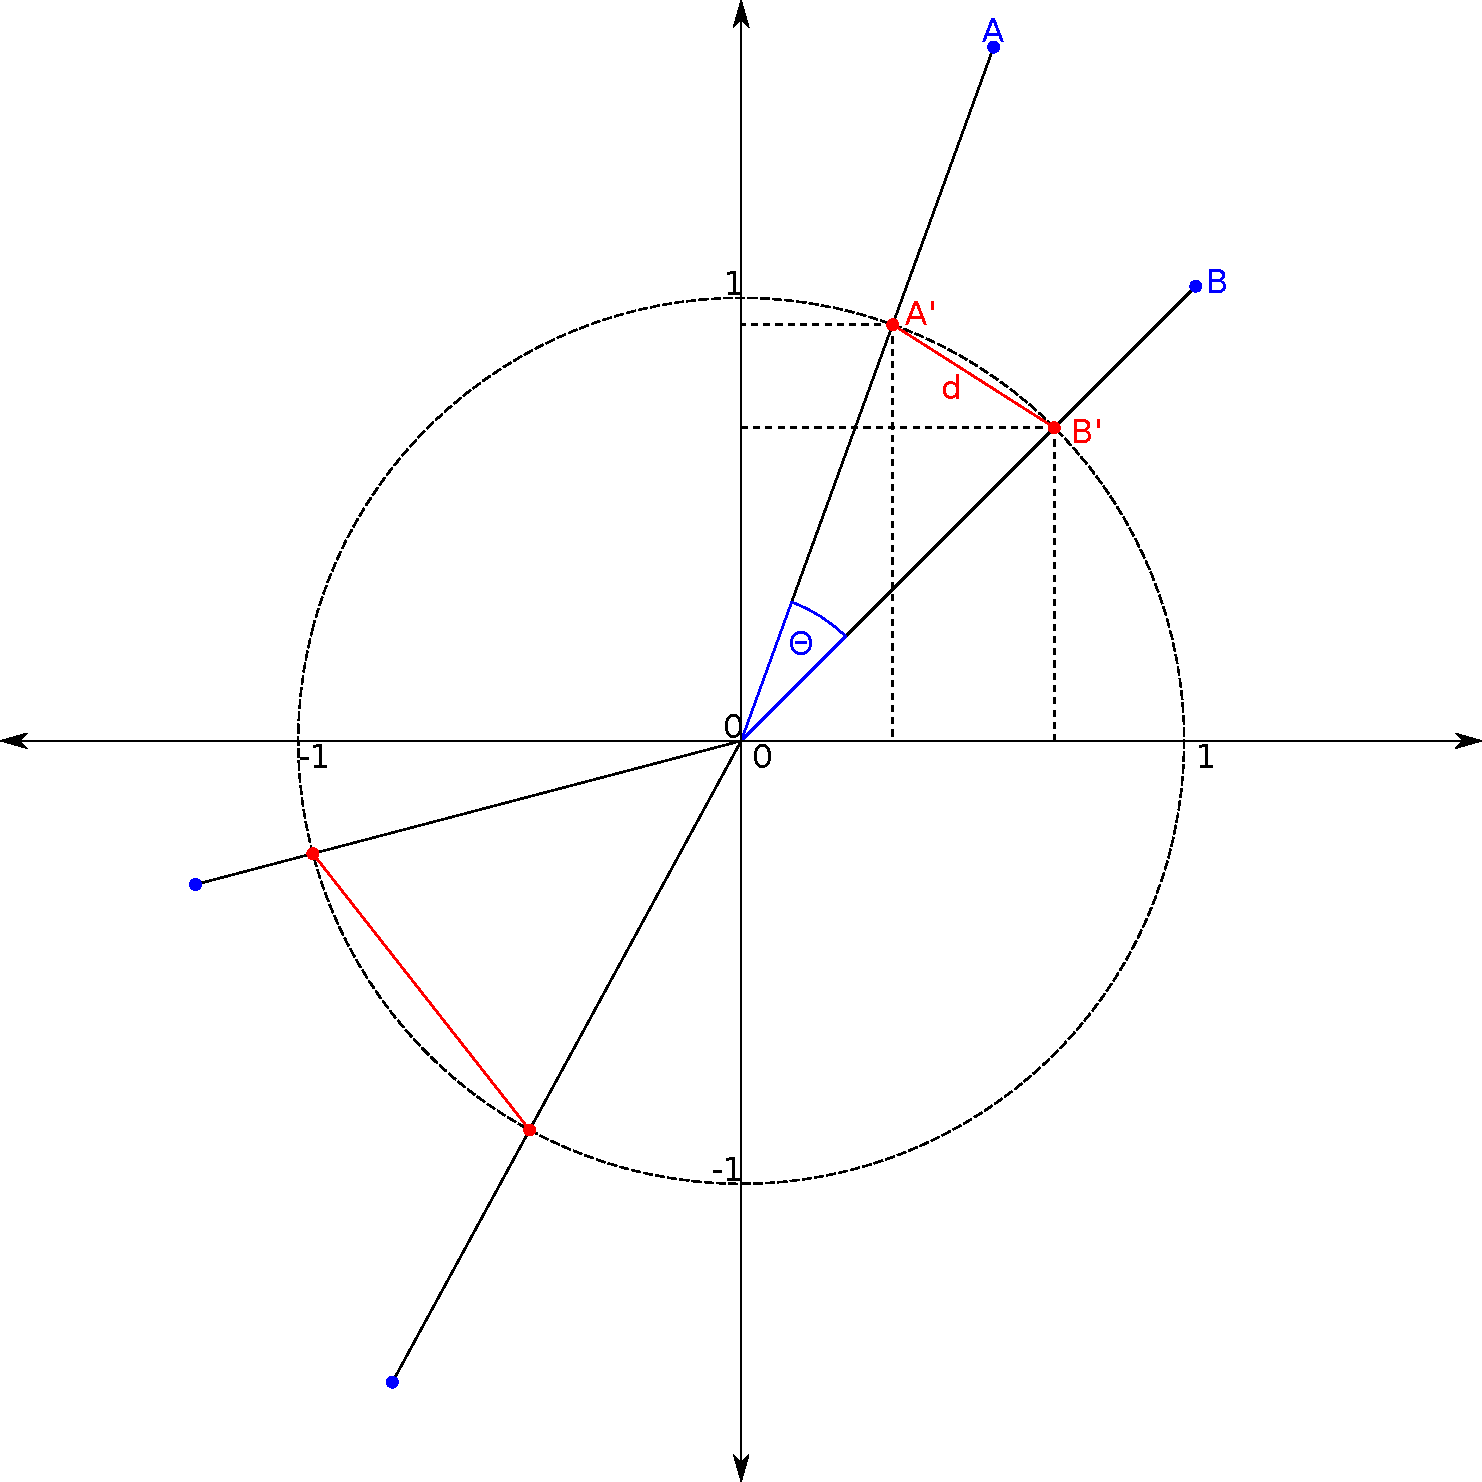
\includegraphics[width=\dimexpr\textwidth-2\fboxsep-2\fboxrule,fbox]{Extra_Graphics/L2_Euclidean.pdf}
    \caption[Mathematical Background of L2 Normalisation]{\textbf{Mathematical Background of L2 Normalisation.} .}
    \label{fig:L2_Normalisation_Background}
\end{figure}

\blindtext

\begin{figure}
    \centering
    \begin{adjustbox}{minipage=\dimexpr\textwidth-2\fboxsep-2\fboxrule,fbox}
        \begin{subfigure}[b]{0.475\textwidth}
            \caption[Dimension Reduction with \Acrshort{PCA}]{\textbf{Dimension Reduction with \Acrshort{PCA}}}
            \label{subfig:Normalisation_PCA}            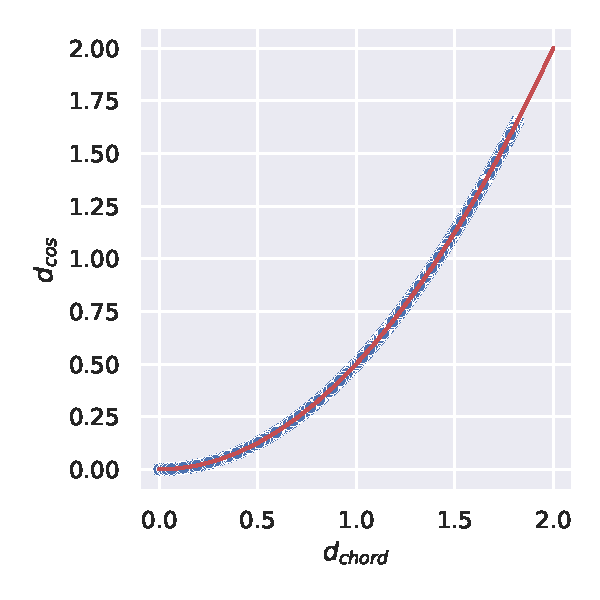
\includegraphics[width=\textwidth]{PCA/Difference_Distance_Calculation.pdf}
        \end{subfigure}
        \hfill
        \begin{subfigure}[b]{0.475\textwidth}
            \caption[Dimension Reduction with \Acrshort{UMAP}]{\textbf{Dimension Reduction with \Acrshort{UMAP}}}
            \label{subfig:Normalisation_UMAP}            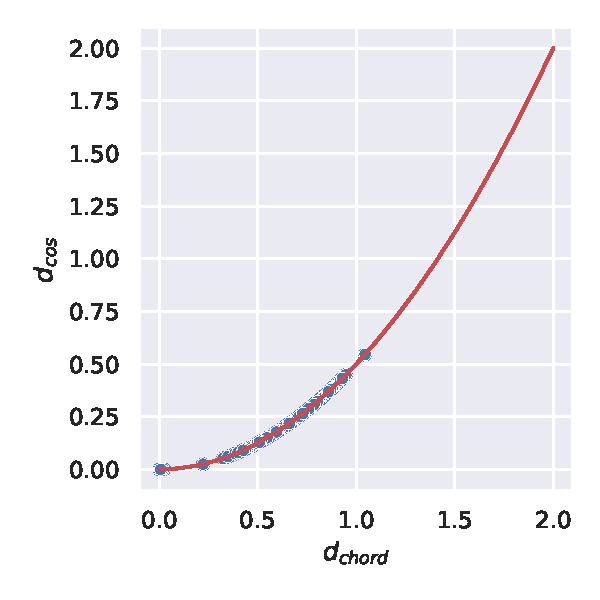
\includegraphics[width=\textwidth]{UMAP/Difference_Distance_Calculation.pdf}
        \end{subfigure}
    \end{adjustbox}
    \caption[Cosine Distance Approximation with L2 Normalisation]{\textbf{Cosine Distance Approximation with L2 Normalisation.} .}
    \label{fig:Normalisation_Methods}
\end{figure}

\blindtext

\blindtext

\section{HDBSCAN} \label{sec:HDBSCAN}

\blindtext

\autocite{mcinnes_hdbscan_2017}
\autocite{malzer_hybrid_2020}

\section{Kneedle} \label{sec:Kneedle}

\blindtext

\autocite{satopaa_finding_2011}

\section{MAFFT} \label{sec:Clustering_Pipeline}

\blindtext
\autocite{katoh_mafft_2013}
\autocite{cock_biopython_2009}

The parameters used in this project with settings varying from the default are listed below. All available settings can be fount in the \href{https://mafft.cbrc.jp/alignment/software/}{manual}

\begin{leftbar}
    %\textbf{mafft}
    \textbf{Bio.Align.Applications.MafftCommandline}
    \begin{nstabbing}
        \qquad\qquad\qquad\qquad\qquad\quad\=\kill
    
        treeout \> (default: off)\\
        
        thread \> (default: 1)\\
        
        input \>
        
        %-{}-{}6merpair \> (default: on)\\
        %\> input\\
        %> \> output
    \end{nstabbing}
\end{leftbar}



\section{Pipeline} \label{sec:Analysis_Pipeline}

\blindtext

\begin{figure}[!hbt]
    \centering
    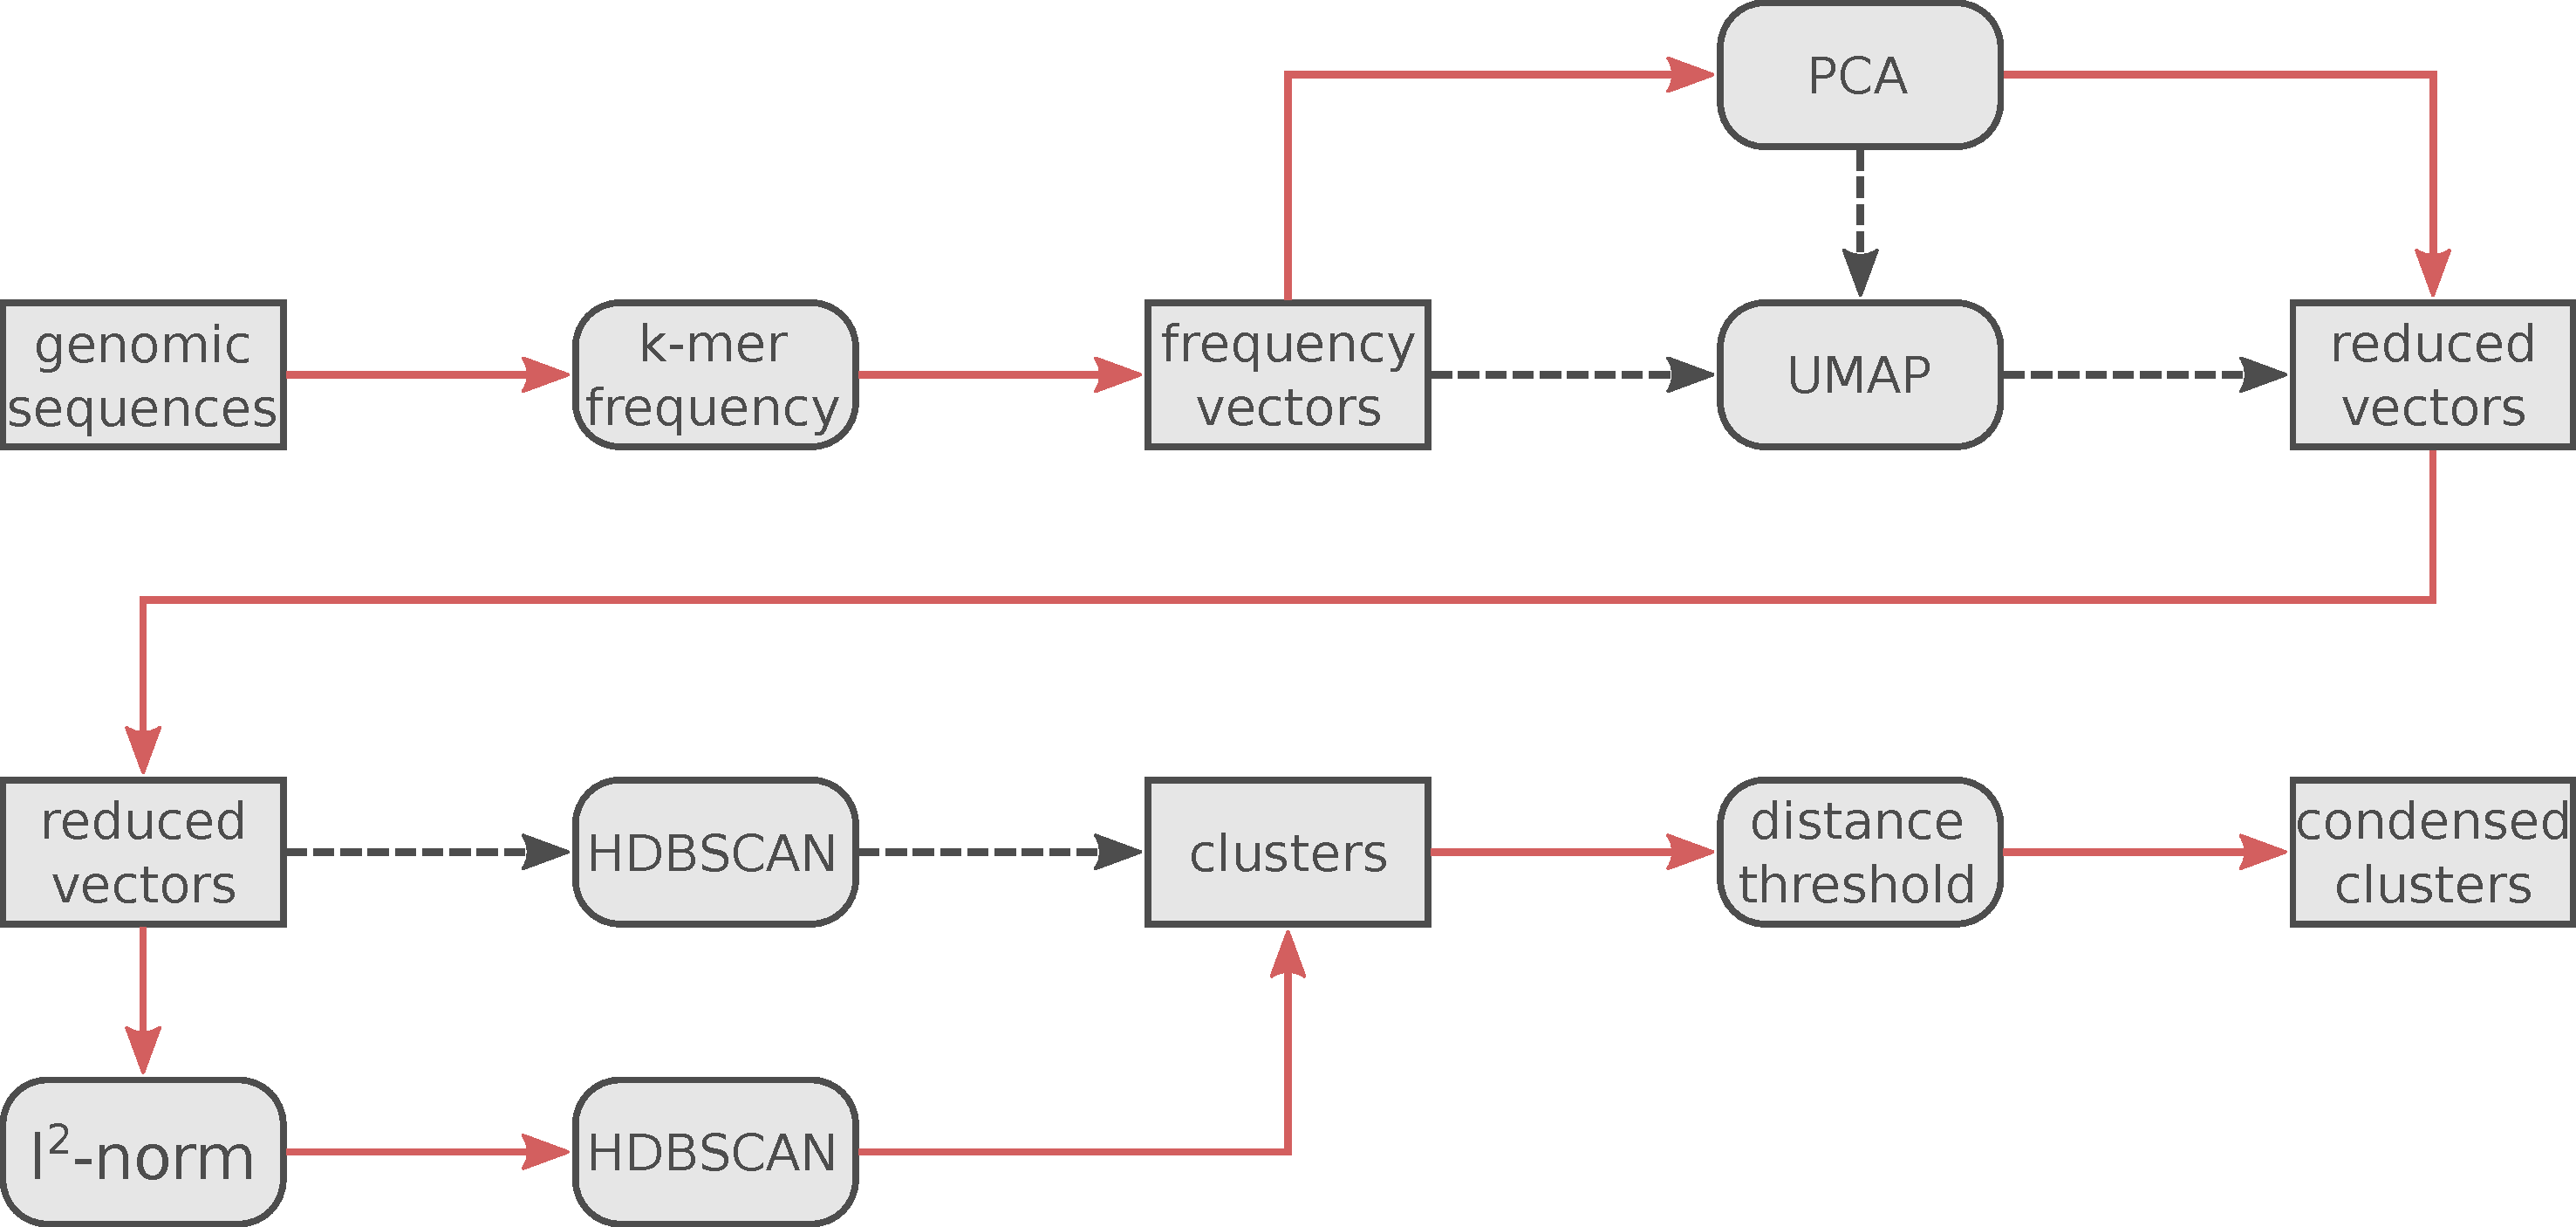
\includegraphics[width=\textwidth]{Graphics/Pipeline_V2.pdf}
    \caption[Clustering Pipeline]{\textbf{Clustering Pipeline.} .}
    \label{fig:Clustering_Pipeline}
\end{figure}

\begin{table}[!hbt]
    \centering
    \caption[Explained Variance by different PCA settings]{\textbf{Explained Variance by different PCA settings.}.}
    \label{tab:PCA_Dimension}
    \pgfplotstabletypeset[
        every head row/.style={
            before row={
                \toprule
            },
            after row={
                \midrule
            },
        },
        every last row/.style={
            after row={
                \bottomrule
            },
        },
        begin table=\begin{tabular*}{.5\textwidth},
        end table=\end{tabular*},
        columns={0,1},
        columns/0/.style={int detect, multicolumn names=l,column name=\textbf{\#Components}, column type=@{\extracolsep{\fill}\hspace{6pt}}r},
        columns/1/.style={multicolumn names=l,column name=\textbf{Explained Variance}, column type=r}
    ]
    {Graphics/PCA.csv}
\end{table}